\setlength{\tabcolsep}{1pt}
\begin{figure}[h]
    \footnotesize
    \small
    \begin{tabularx}{\columnwidth}{ YYYYYY }
        % \cline{2-7}
        %    \multicolumn{1}{c|}{} 
        %  & \multicolumn{3}{c|}{Fantastical aardvarks}  
        %  & \multicolumn{3}{c|}{Spelunking elephants}\\
        % \hline
        %  Foo bar & A & B & C & A & B & C\\
        Input & \ptopzero &  \nulltext &  \directinversion &  \negprox &  \method \\
        \multicolumn{6}{c}{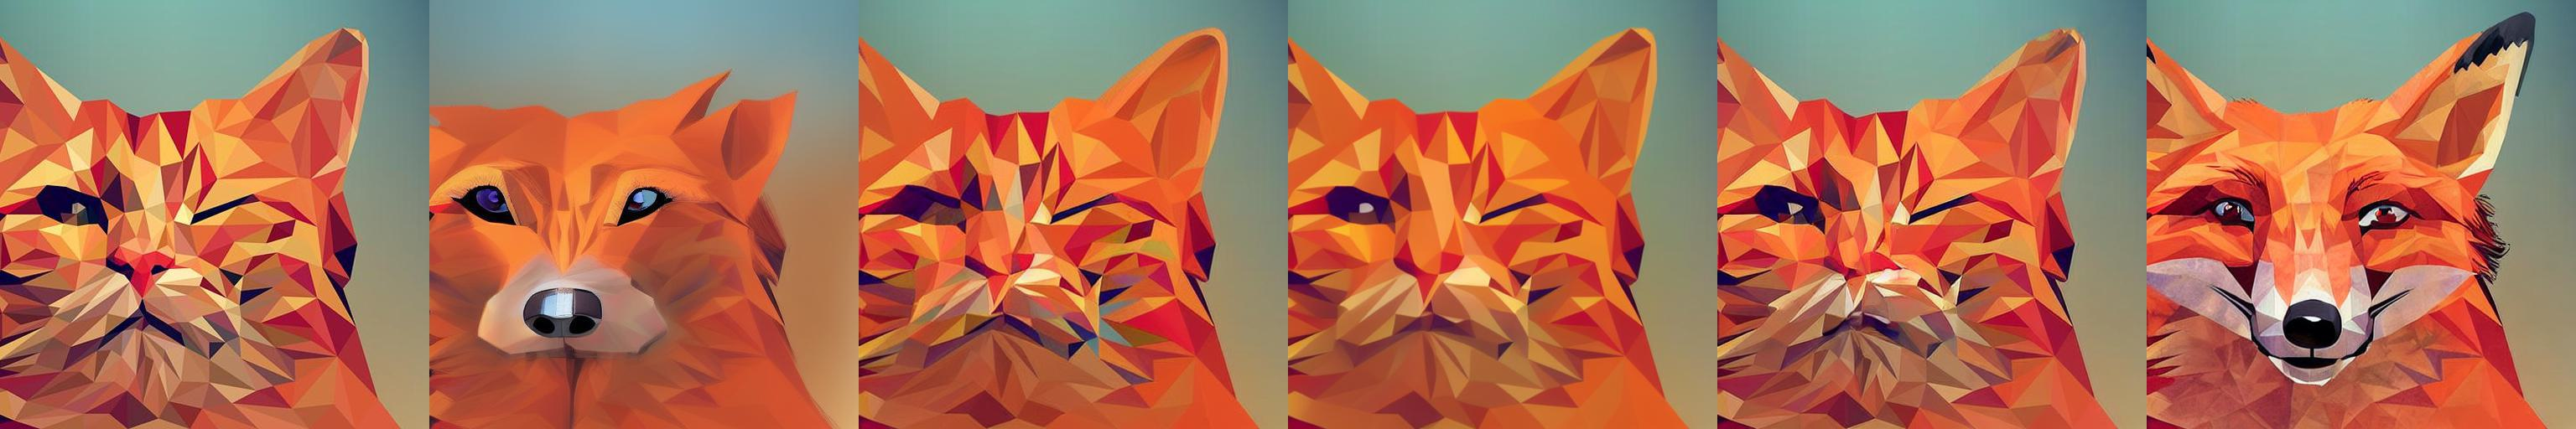
\includegraphics[width=\columnwidth]{fig/ex_all/0_random_140-000000000080}} \\
        \multicolumn{6}{c}{``\textit{a \textcolor{BrickRed}{\st{cat}} \textcolor{RoyalBlue}{\textbf{fox}} is shown in a low polygonal style}"} \\
        \multicolumn{6}{c}{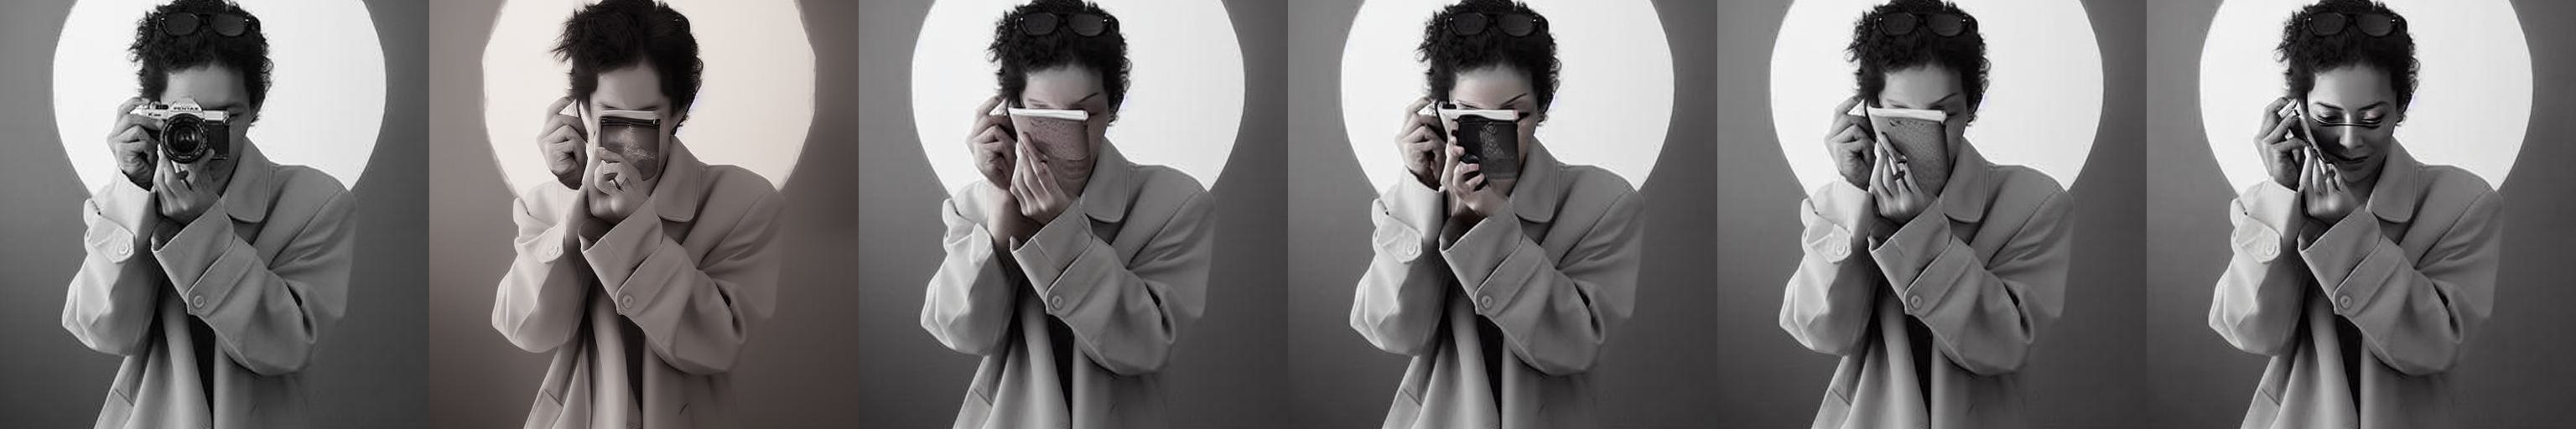
\includegraphics[width=\columnwidth]{fig/ex_all/1_change_object_80-2_natural-2_human-122000000002}} \\
        \multicolumn{6}{c}{``\textit{a woman in a coat holding a \textcolor{BrickRed}{\st{camera}} \textcolor{RoyalBlue}{\textbf{phone}} on white plate}"} \\
        \multicolumn{6}{c}{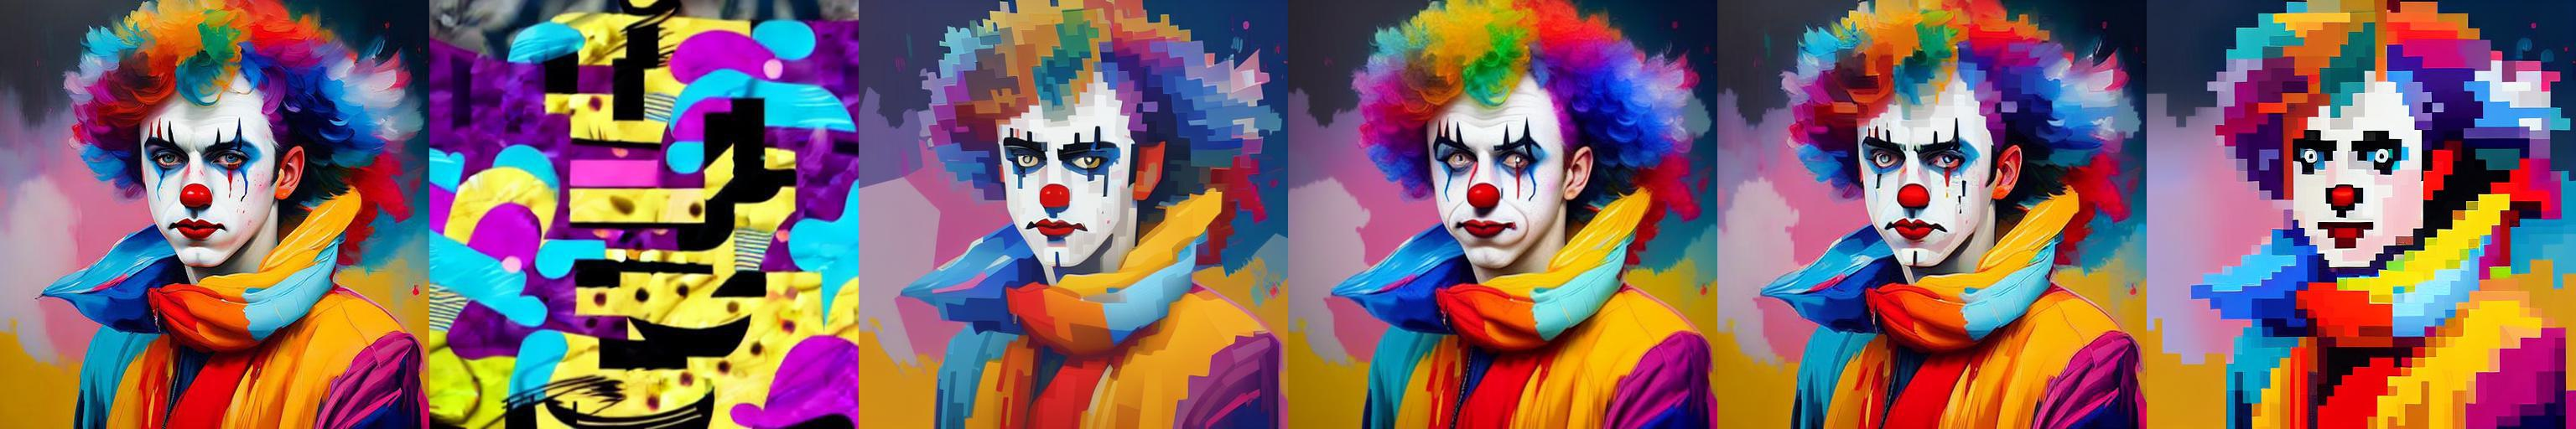
\includegraphics[width=\columnwidth]{fig/ex_all/9_change_style_80-1_artificial-2_human-912000000001}} \\
        \multicolumn{6}{c}{``\textit{a clown \textcolor{RoyalBlue}{\textbf{in pixel art style}} with colorful hair}"} \\
        \multicolumn{6}{c}{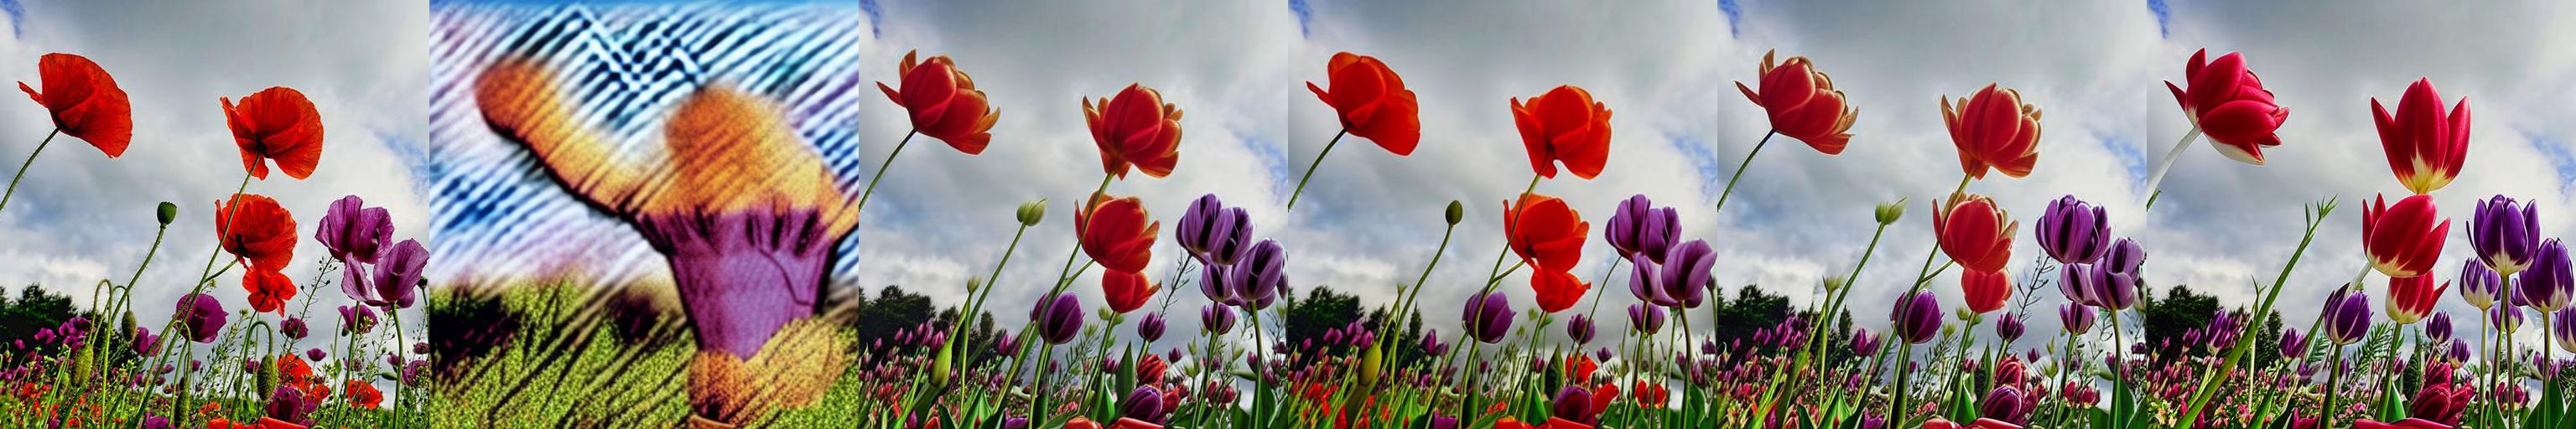
\includegraphics[width=\columnwidth]{fig/ex_all/0_random_140-000000000101}} \\
        \multicolumn{6}{c}{``\textit{\textcolor{BrickRed}{\st{poppies}} \textcolor{RoyalBlue}{\textbf{tulips}}}"} \\
        \multicolumn{6}{c}{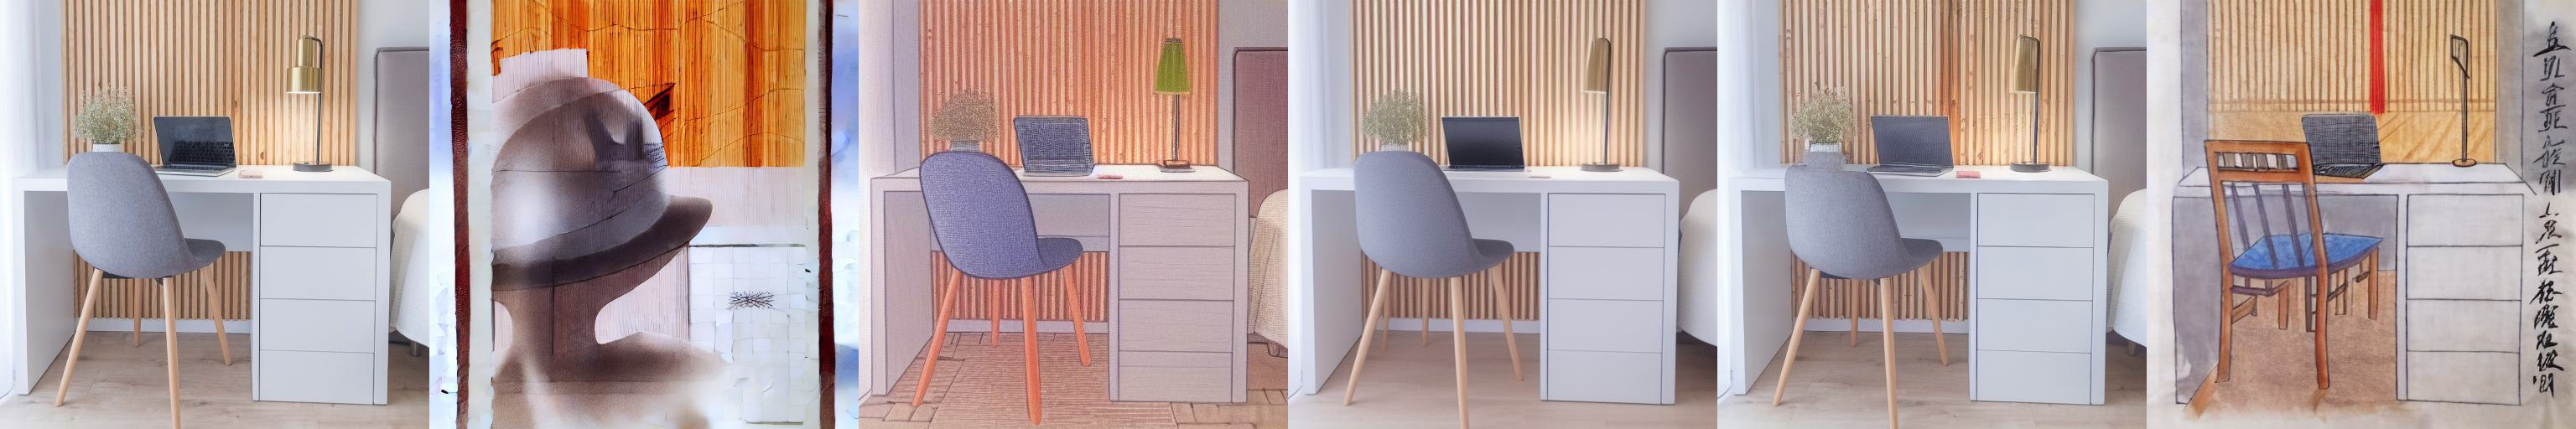
\includegraphics[width=\columnwidth]{fig/ex_all/9_change_style_80-2_natural-3_indoor-923000000007}} \\
        \multicolumn{6}{c}{``\textit{\textcolor{RoyalBlue}{\textbf{chinese painting of}} a white desk with a laptop and chair}"} \\
        \end{tabularx}
        \caption{Examples from the PieBench dataset illustrating the strengths of \method{}, including superior style transfer, content modification, and object removal.        }
    \label{fig:qual_adv}
  \end{figure}